% ai-helper issue #46: what we learned from Kento's SBND YZ map file.
% Figures and numbers: ../scripts/make_deck_figs.py <map.root> deck-figs
%   (numbers in deck-figs/deck_numbers.json); plane-comparison and validation
%   numbers from ../46-sbnd-yz-depo-scaling.md sections 1 and 3
%   (../figs/plane_compare.json, ../figs/detsim_scaling.json).
% Build (twice): pdflatex 46-yz-map-file-summary.tex
\documentclass[aspectratio=169,10pt]{beamer}
\usetheme{default}
\setbeamertemplate{navigation symbols}{}
\setbeamertemplate{footline}{\hfill\scriptsize\color{gray}ai-helper \#46 \quad \insertframenumber/\inserttotalframenumber\hspace*{4mm}\vspace*{2mm}}
\setbeamertemplate{itemize items}{\textbullet}
\setbeamertemplate{itemize subitem}{--}
\setbeamerfont{frametitle}{size=\large,series=\bfseries}
\setbeamercolor{frametitle}{fg=black}
\setbeamercolor{structure}{fg=black!75}
\usepackage[T1]{fontenc}
\usepackage{lmodern}
\usepackage{booktabs}
\usepackage{graphicx}
\usepackage{xcolor}
\graphicspath{{deck-figs/}}
\definecolor{open}{HTML}{B5470B}
\newcommand{\open}[1]{\textcolor{open}{\textbf{#1}}}
\newcommand{\code}[1]{\texttt{#1}}
\setlength{\tabcolsep}{4pt}
% tighter lists
\makeatletter
\def\@listi{\leftmargin\leftmargini \topsep 2pt \parsep 0pt \itemsep 3pt}
\let\@listI\@listi
\def\@listii{\leftmargin\leftmarginii \topsep 1pt \parsep 0pt \itemsep 1pt}
\makeatother
\setlength{\leftmargini}{1.3em}
\setlength{\leftmarginii}{1.2em}

\title{SBND YZ non-uniformity map\\for the Wire-Cell simulation}
\subtitle{What we learned from Kento's map file}
\author{ai-helper issue \#46}
\date{2026-11-24}

\begin{document}

% ---------------------------------------------------------------- 1
\begin{frame}
\titlepage
\vspace{-6mm}
\begin{center}\footnotesize\color{gray}
Input: \code{run\_2\_gen\_2\_BNBLight\_data\_v10\_14\_02\_02\_200usEast80usWest.root}\\
Figures and numbers: \code{scripts/make\_deck\_figs.py}, \code{scripts/compare\_planes.py},\\
issue doc \code{46-sbnd-yz-depo-scaling.md} sections 1--3
\end{center}
\end{frame}

% ---------------------------------------------------------------- 2
\begin{frame}{The file}
\begin{columns}[T]
\begin{column}{0.5\textwidth}
\textbf{Provenance}
\begin{itemize}
\item From Kento, received 2026-11-12.
\item ROOT file, 756\,kB, 30 histograms.
\item Data only. No MC histograms in the file.
\end{itemize}
\vspace{3mm}
\textbf{Conventions}
\begin{itemize}
\item Plane $p$: 0 = U, 1 = V, 2 = Y (collection).
\item TPC $t$: 0 = East ($x<0$), 1 = West ($x>0$).
\item 2D maps: x axis = z [cm], y axis = y [cm].
\item 100 $\times$ 80 pixels of 5 $\times$ 5\,cm$^2$: z 0--500\,cm, y $-$200 to 200\,cm.
\end{itemize}
\end{column}
\begin{column}{0.48\textwidth}
\textbf{The file name, as we read it (not confirmed)}
\begin{itemize}
\item \code{run\_2}: SBND Run 2
\item \code{gen\_2}: Gen-2 production
\item \code{BNBLight}: BNB-light data stream
\item \code{v10\_14\_02\_02}: software version
\item \code{200usEast80usWest}: \open{not explained anywhere we have.} Possibly a time or drift cut per TPC. Question for Kento.
\end{itemize}
\end{column}
\end{columns}
\end{frame}

% ---------------------------------------------------------------- 3
\begin{frame}{What is in it}
\centering\small
\begin{tabular}{@{}llll@{}}
\toprule
name ($p$ = plane, $t$ = TPC) & type & title & content \\
\midrule
\code{zy\_p\_t} & TH2F & ``zy (Median of dqdx)'' & median dQ/dx of the hits in a pixel \\
\code{CzyHist\_p\_t} & TH2F & ``zy (Median of dqdx)'' & correction factor $C$ \\
\code{zynhits\_p\_t} & TH2F & ``zy (nhits)'' & hits per pixel \\
\code{zydqdx\_p\_t} & TH2F & ``zy (dqdx)'' & NaN in 806--5160 pixels; ignored \\
\code{dqdxHist\_p\_t} & TH1F & ``dqdx'' & 1D dQ/dx, 200 bins, 200--2000 \\
\bottomrule
\end{tabular}
\raggedright
\vspace{4mm}
\begin{itemize}
\item 6 of each: 3 planes $\times$ 2 TPCs. \code{CzyHist} has the same title as \code{zy} (copied).
\item Unit: the 1D histograms have the axis title ``dQ/dx [ADC/cm]''. The 2D maps carry no unit; we assume the same. \open{To confirm with Kento}, including the calibration stage.
\item \code{zydqdx}: where it is finite, \code{zydqdx}/\code{zynhits} is 1260--1300, so it looks like a per-pixel sum of dQ/dx. The NaNs make it unusable.
\end{itemize}
\end{frame}

% ---------------------------------------------------------------- 4
\begin{frame}{Coverage: hits per pixel (\code{zynhits})}
\begin{columns}[c]
\begin{column}{0.63\textwidth}
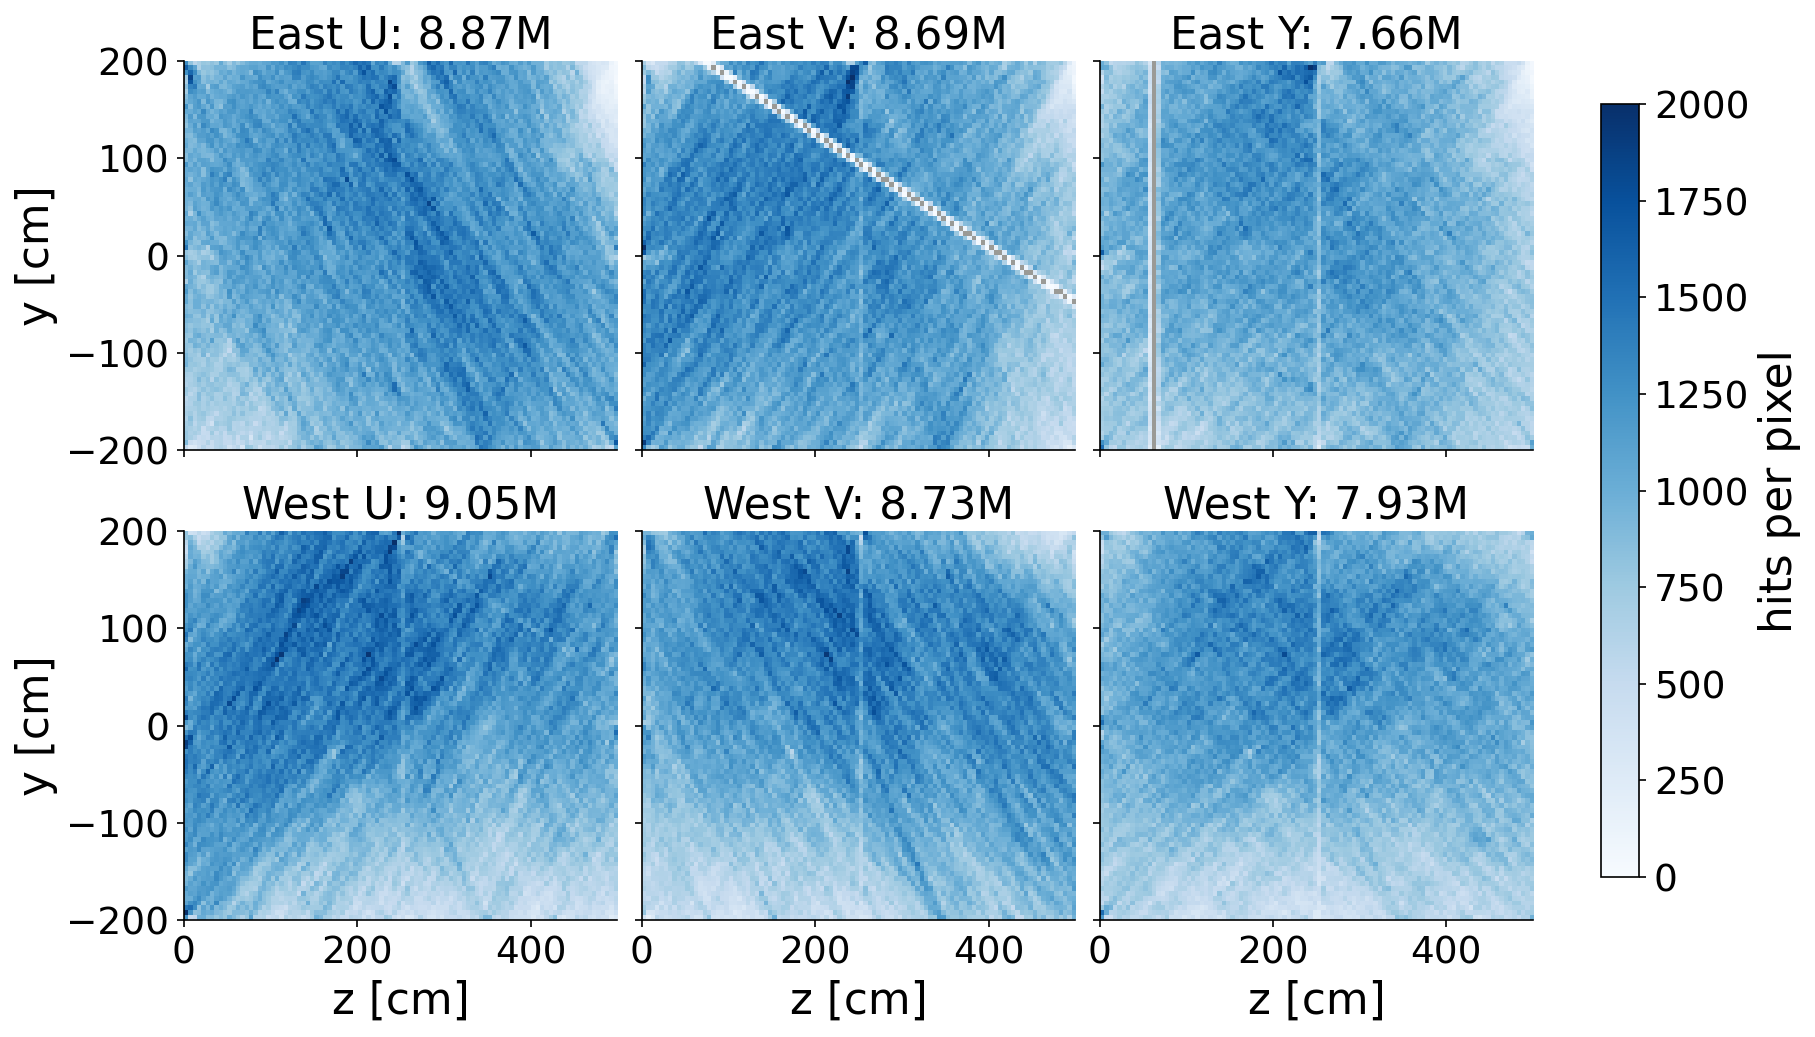
\includegraphics[width=\textwidth]{fig_nhits.png}\\
\footnotesize Gray: empty pixels ($C=0$).
\end{column}
\begin{column}{0.36\textwidth}
\footnotesize\setlength{\tabcolsep}{3pt}
\begin{tabular}{@{}lrrrr@{}}
\toprule
 & hits & median & empty & $<$100 \\
 & & /pixel & & hits \\
\midrule
East U & 8.87\,M & 1132 & 0 & 9 \\
East V & 8.69\,M & 1131 & 52 & 64 \\
East Y & 7.66\,M & 979 & 80 & 6 \\
West U & 9.05\,M & 1171 & 0 & 0 \\
West V & 8.73\,M & 1130 & 0 & 0 \\
West Y & 7.93\,M & 1012 & 0 & 0 \\
\bottomrule
\end{tabular}
\vspace{2mm}
\begin{itemize}
\item East V empty: a diagonal at 60$^\circ$ from vertical (the V wire direction), z 80--500\,cm.
\item East Y empty: one full column, z = 60--65\,cm.
\item West: at least 163--252 hits in every pixel.
\end{itemize}
\end{column}
\end{columns}
\end{frame}

% ---------------------------------------------------------------- 5a
\begin{frame}{The variables, East U (plane 0, TPC 0)}
\centering
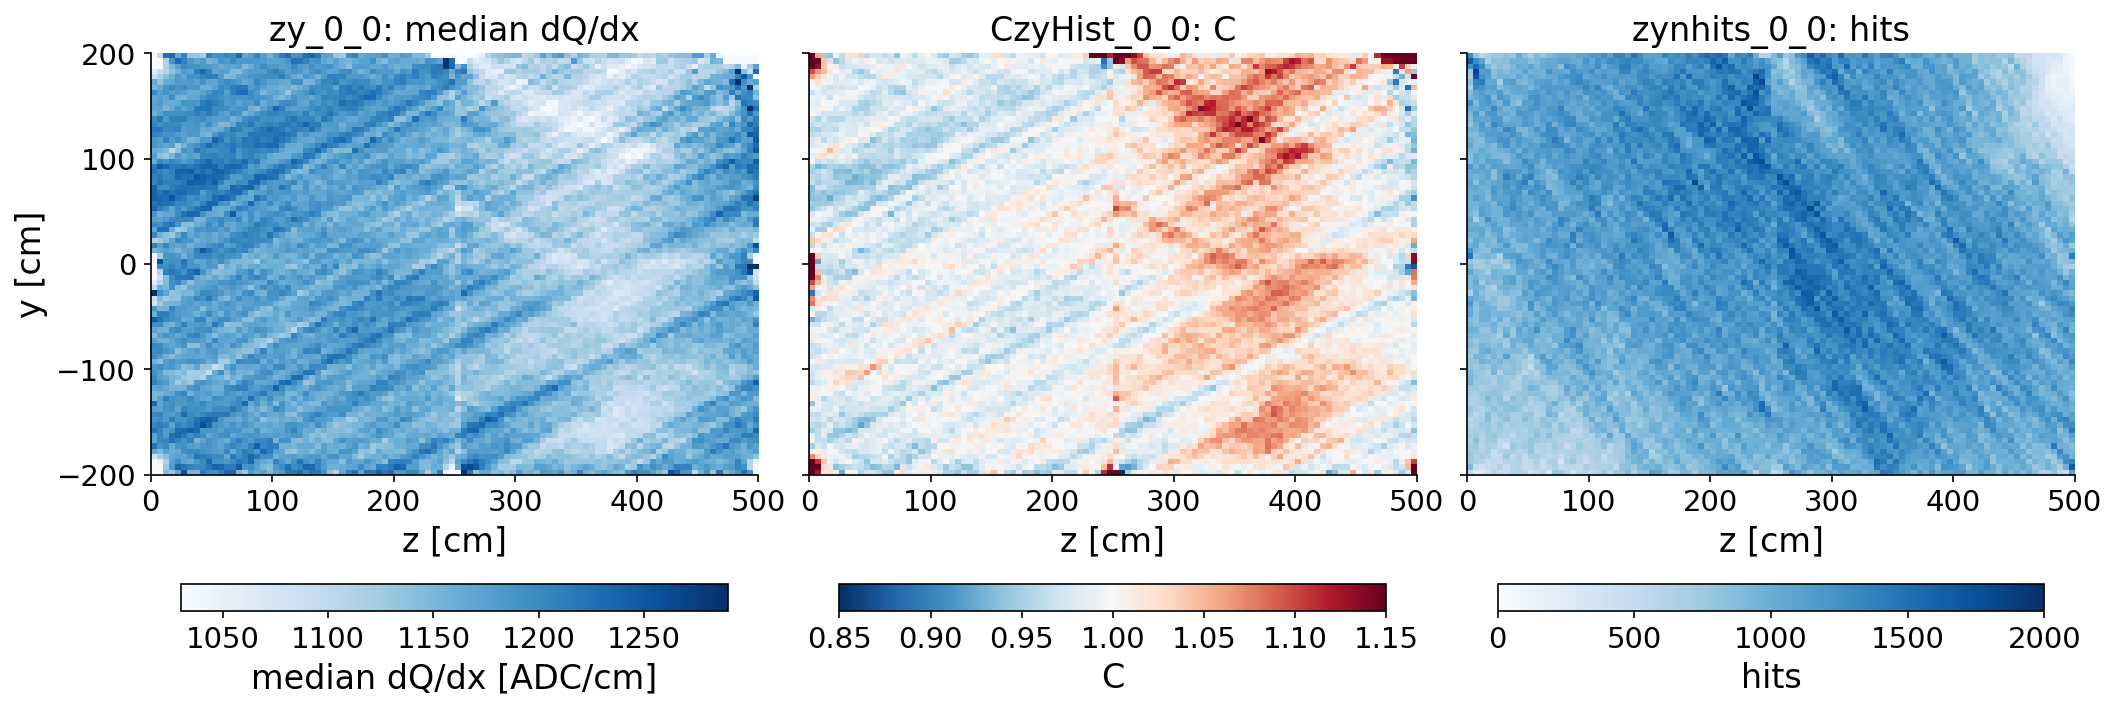
\includegraphics[width=0.96\textwidth]{fig_vars_EastU.png}
\raggedright
\begin{itemize}
\item For every pixel with data, $\mathtt{zy}\times C = M$, the median of \code{zy} over the pixels of that plane and TPC (checked on all six: equal within $1.2\times10^{-7}$, relative). So $g = 1/C = \mathtt{zy}/M$, the pixel's response relative to the plane median. $C = 0$ (gray) where there is no data.
\item $M$ = 1160\,ADC/cm. $C$ from 0.85 to 1.92; $g$ (normalized) rms 3.8\,\%.
\item Hits per pixel: min 20, median 1132, max 1842. Empty pixels: none; pixels with $<$100 hits: 9.
\end{itemize}
\end{frame}

% ---------------------------------------------------------------- 5b
\begin{frame}{The variables, East V (plane 1, TPC 0)}
\centering
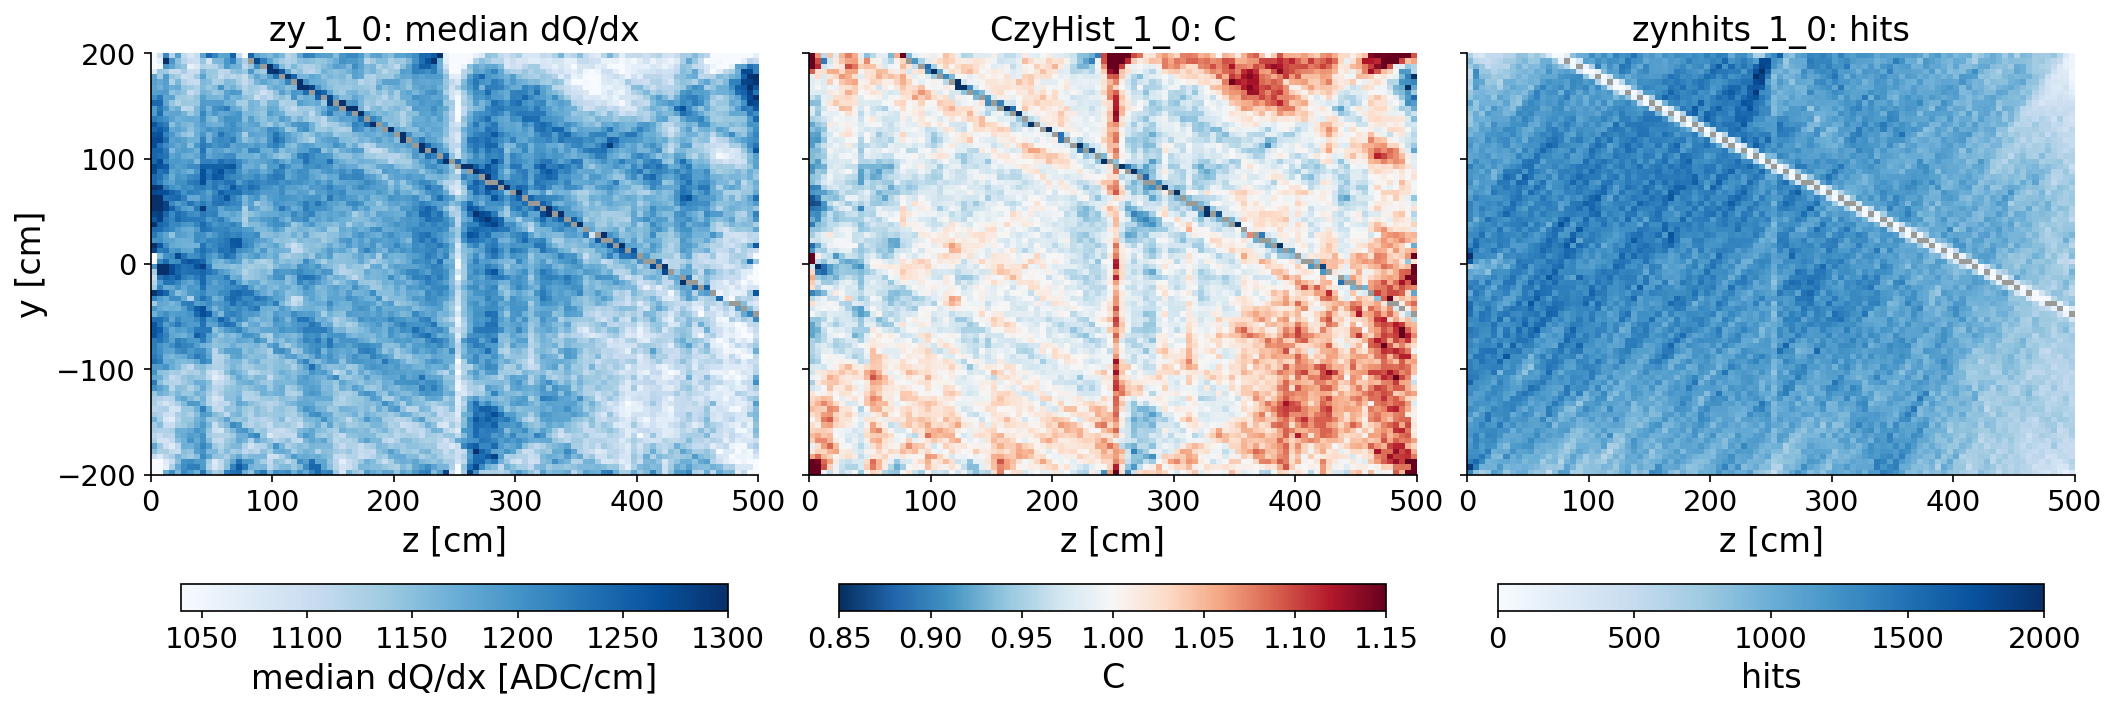
\includegraphics[width=0.96\textwidth]{fig_vars_EastV.png}
\raggedright
\begin{itemize}
\item Same variables as the first of these slides: $\mathtt{zy}\times C = M$, $g = 1/C = \mathtt{zy}/M$; gray = no data ($C=0$).
\item $M$ = 1164\,ADC/cm. $C$ from 0.60 to 1.84; $g$ (normalized) rms 4.6\,\%.
\item Hits per pixel: min 2, median 1130, max 2064. Empty pixels: 52; pixels with $<$100 hits: 64.
\end{itemize}
\end{frame}

% ---------------------------------------------------------------- 5c
\begin{frame}{The variables, East Y (plane 2, TPC 0)}
\centering
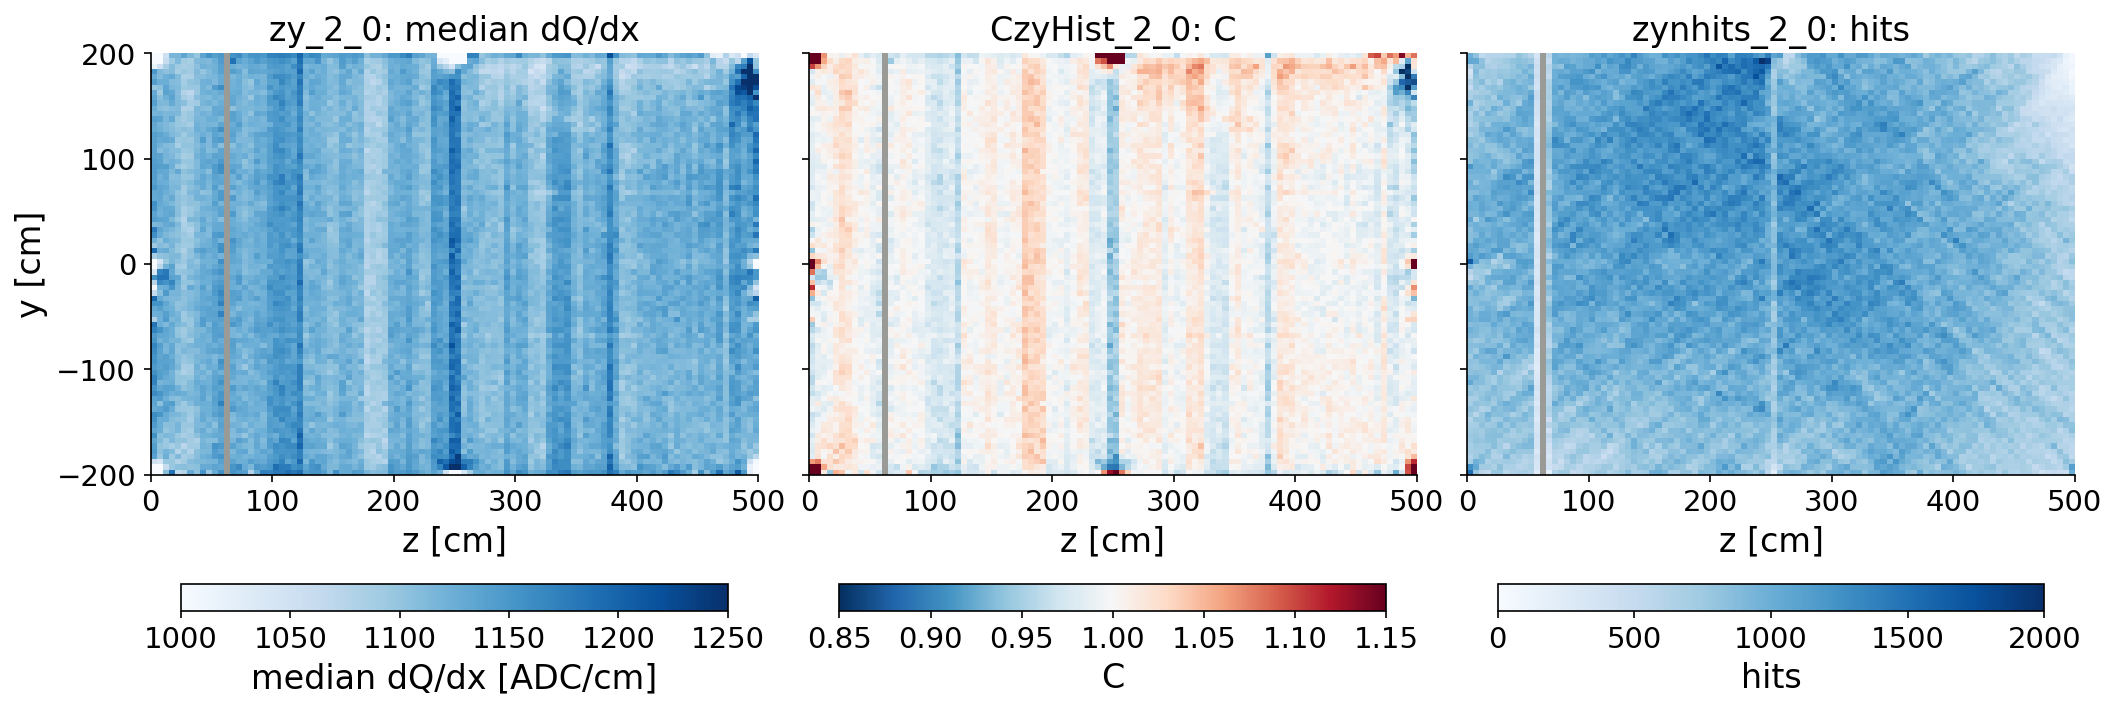
\includegraphics[width=0.96\textwidth]{fig_vars_EastY.png}
\raggedright
\begin{itemize}
\item Same variables as the first of these slides: $\mathtt{zy}\times C = M$, $g = 1/C = \mathtt{zy}/M$; gray = no data ($C=0$).
\item $M$ = 1121\,ADC/cm. $C$ from 0.79 to 2.21; $g$ (normalized) rms 2.7\,\%.
\item Hits per pixel: min 45, median 979, max 2122. Empty pixels: 80; pixels with $<$100 hits: 6.
\end{itemize}
\end{frame}

% ---------------------------------------------------------------- 5d
\begin{frame}{The variables, West U (plane 0, TPC 1)}
\centering
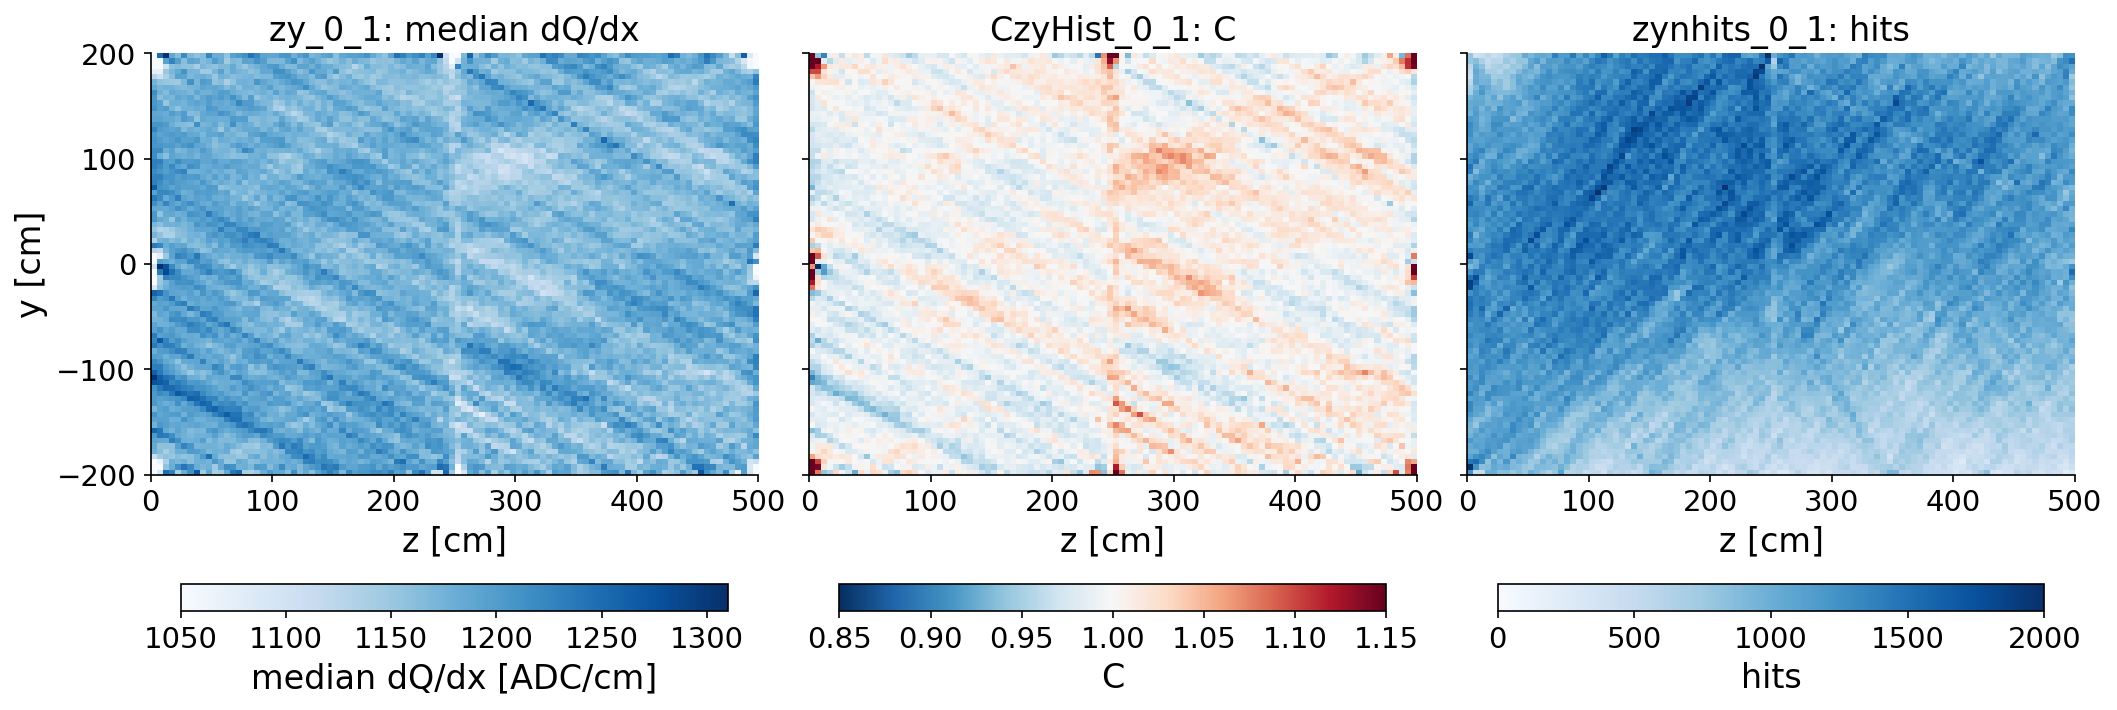
\includegraphics[width=0.96\textwidth]{fig_vars_WestU.png}
\raggedright
\begin{itemize}
\item Same variables as the first of these slides: $\mathtt{zy}\times C = M$, $g = 1/C = \mathtt{zy}/M$; gray = no data ($C=0$).
\item $M$ = 1175\,ADC/cm. $C$ from 0.84 to 1.99; $g$ (normalized) rms 2.6\,\%.
\item Hits per pixel: min 229, median 1171, max 2309. Empty pixels: none; pixels with $<$100 hits: 0.
\end{itemize}
\end{frame}

% ---------------------------------------------------------------- 5e
\begin{frame}{The variables, West V (plane 1, TPC 1)}
\centering
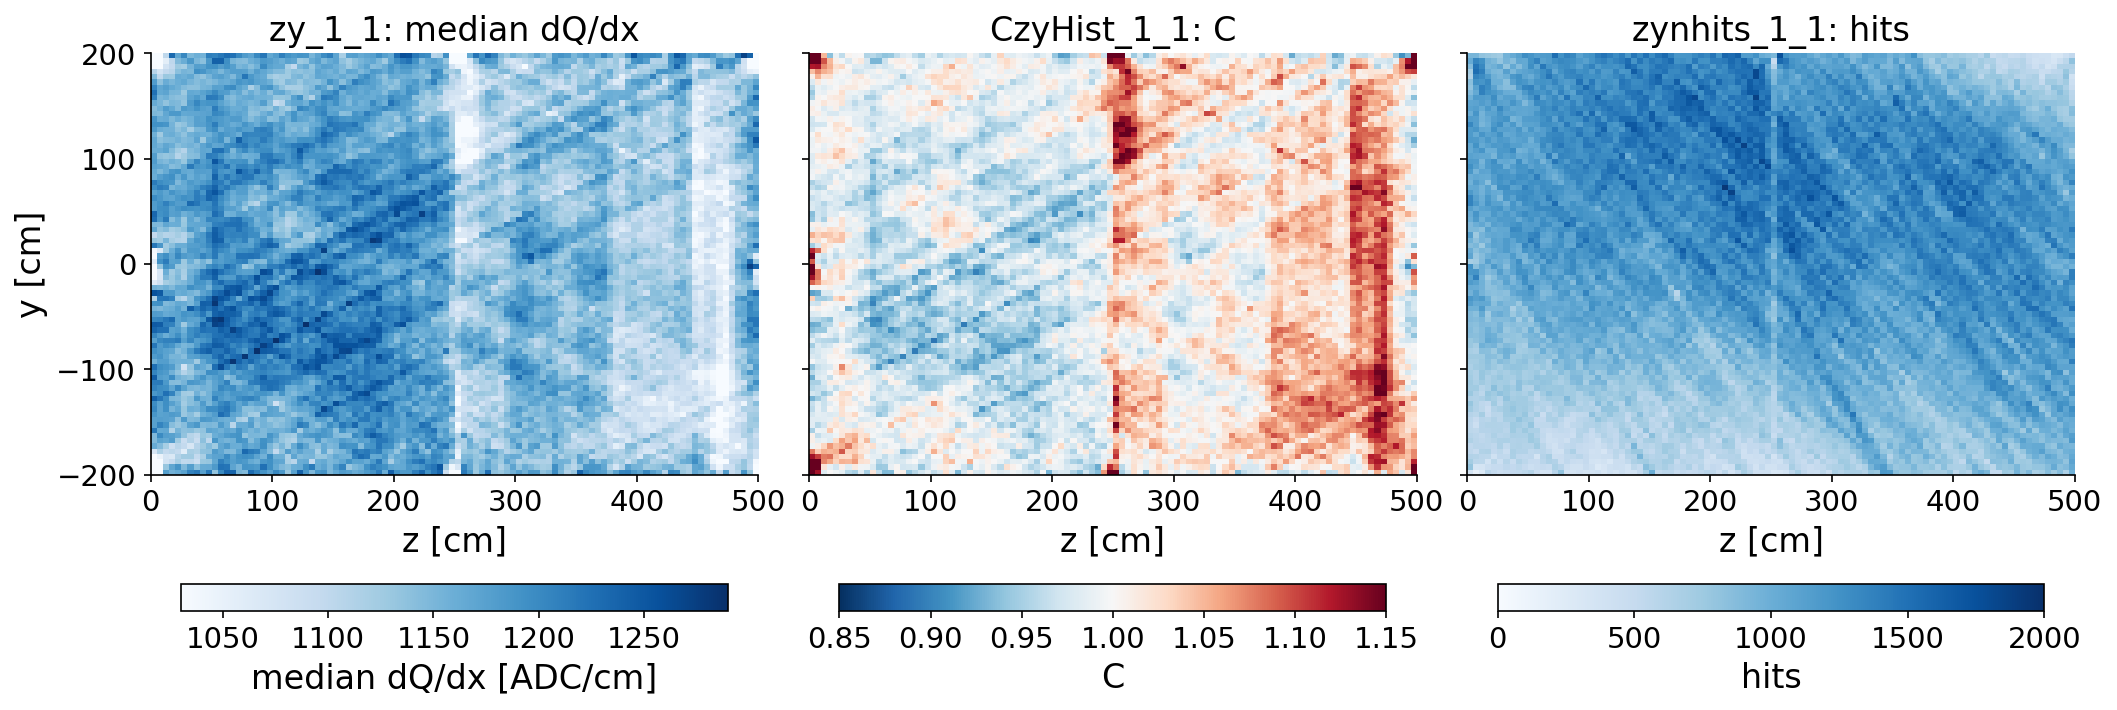
\includegraphics[width=0.96\textwidth]{fig_vars_WestV.png}
\raggedright
\begin{itemize}
\item Same variables as the first of these slides: $\mathtt{zy}\times C = M$, $g = 1/C = \mathtt{zy}/M$; gray = no data ($C=0$).
\item $M$ = 1156\,ADC/cm. $C$ from 0.89 to 1.69; $g$ (normalized) rms 4.4\,\%.
\item Hits per pixel: min 163, median 1130, max 1935. Empty pixels: none; pixels with $<$100 hits: 0.
\end{itemize}
\end{frame}

% ---------------------------------------------------------------- 5f
\begin{frame}{The variables, West Y (plane 2, TPC 1)}
\centering
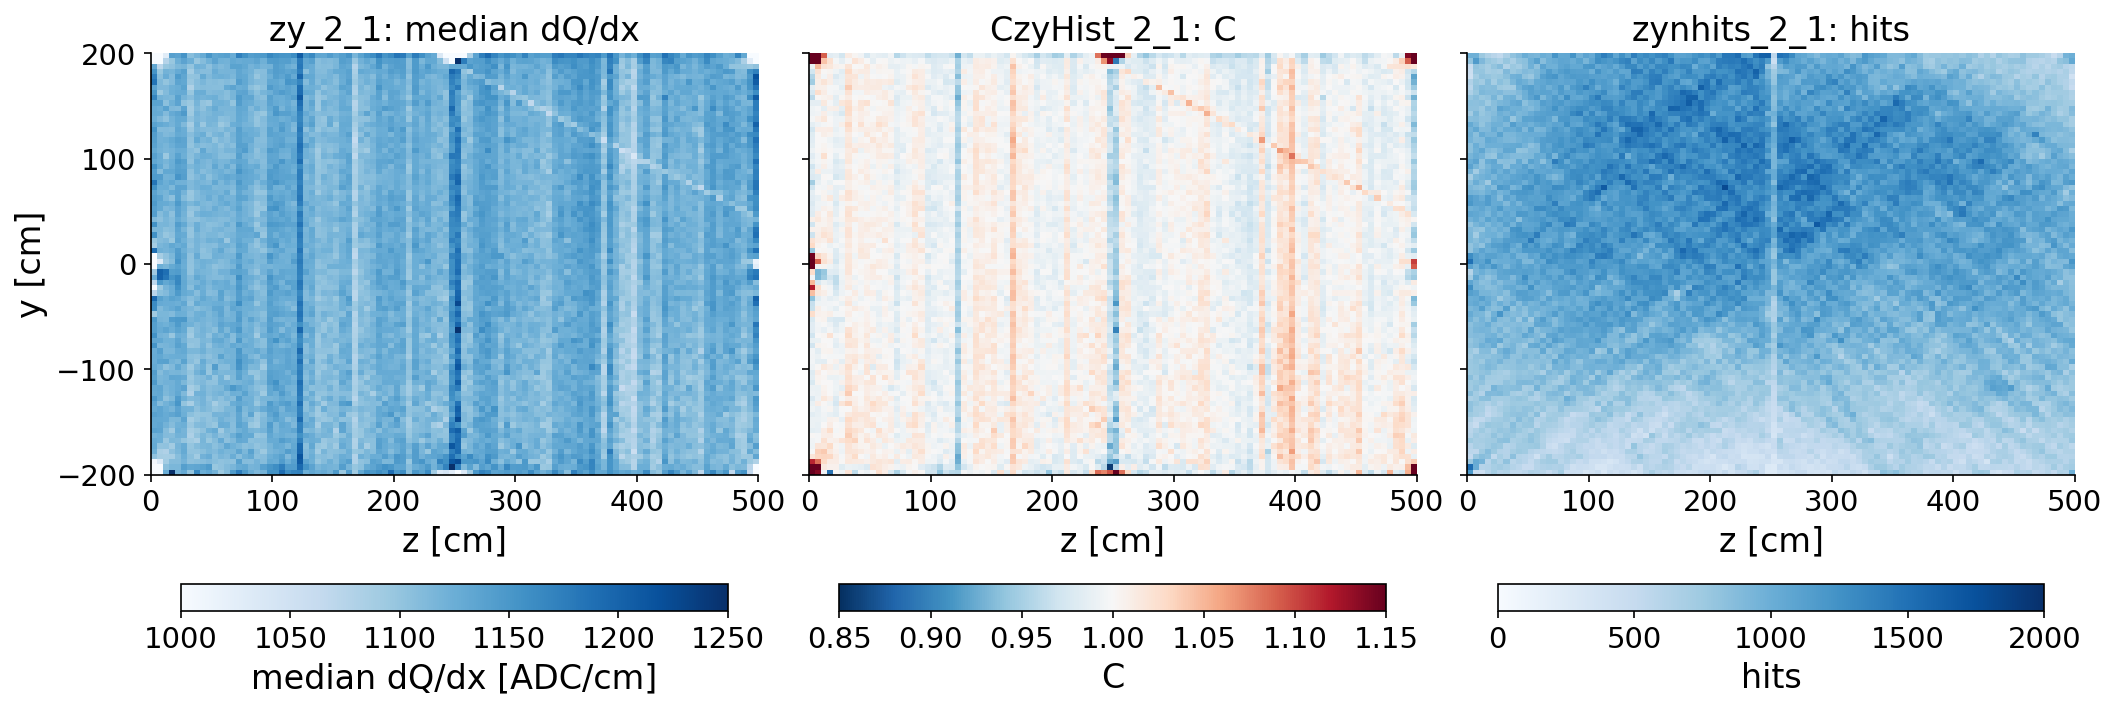
\includegraphics[width=0.96\textwidth]{fig_vars_WestY.png}
\raggedright
\begin{itemize}
\item Same variables as the first of these slides: $\mathtt{zy}\times C = M$, $g = 1/C = \mathtt{zy}/M$; gray = no data ($C=0$).
\item $M$ = 1121\,ADC/cm. $C$ from 0.86 to 2.38; $g$ (normalized) rms 2.4\,\%.
\item Hits per pixel: min 252, median 1012, max 1793. Empty pixels: none; pixels with $<$100 hits: 0.
\end{itemize}
\end{frame}

% ---------------------------------------------------------------- 6
\begin{frame}{How the map is used in the simulation (doc section 2)}
\small
\begin{columns}[T]
\begin{column}{0.5\textwidth}
\textbf{Converter} \code{gen/test/convert-yzmap-sbnd.py}
\begin{itemize}
\item Factor $g = 1/C$ per plane and TPC.
\item \code{inv-norm} (default): $g$ divided by its mean over the pixels with data. Mean 1, so the overall charge scale is kept. The raw mean is 0.9955--1.0009: a change of $<$0.5\,\%.
\item Empty pixels get 1 (no YZ effect). Dead channels are the channel-status database's job.
\item Keys: \code{AnodePlane:apa0} = East, \code{apa1} = West.
\item YZMap: nbinsz 100, nbinsy 80, 5\,cm $\times$ 5\,cm, zoffset 0, yoffset 200\,cm.
\item Output, 80\,kB, in wire-cell-data (acbe8e5):\\ {\footnotesize\code{sbnd-yzmap-run2-gen2-bnblight-v1.json.bz2}}
\end{itemize}
\end{column}
\begin{column}{0.48\textwidth}
\textbf{\code{Gen::DepoTransformYZ}} (WCT branch \code{sbnd-yz-depo-scaling})
\begin{itemize}
\item A \code{DepoTransform} that overrides \code{modify\_depo(WirePlaneId, depo)}.
\item Every depo, every plane: charge $\times\,g$(plane, TPC, z, y) before that plane's \code{BinnedDiffusion}.
\item Each plane gets its own factor at no extra cost.
\item \code{configure()} fails if the map has no non-zero value for a plane of the anode.
\item SimChannels are written upstream: unscaled.
\item Also fixed: \code{YZMap} read one past the end of the grid at the upper y or z edge.
\end{itemize}
\end{column}
\end{columns}
\end{frame}

% ---------------------------------------------------------------- 7
\begin{frame}{Non-uniformity maps: $g$ normalized to mean 1}
\centering
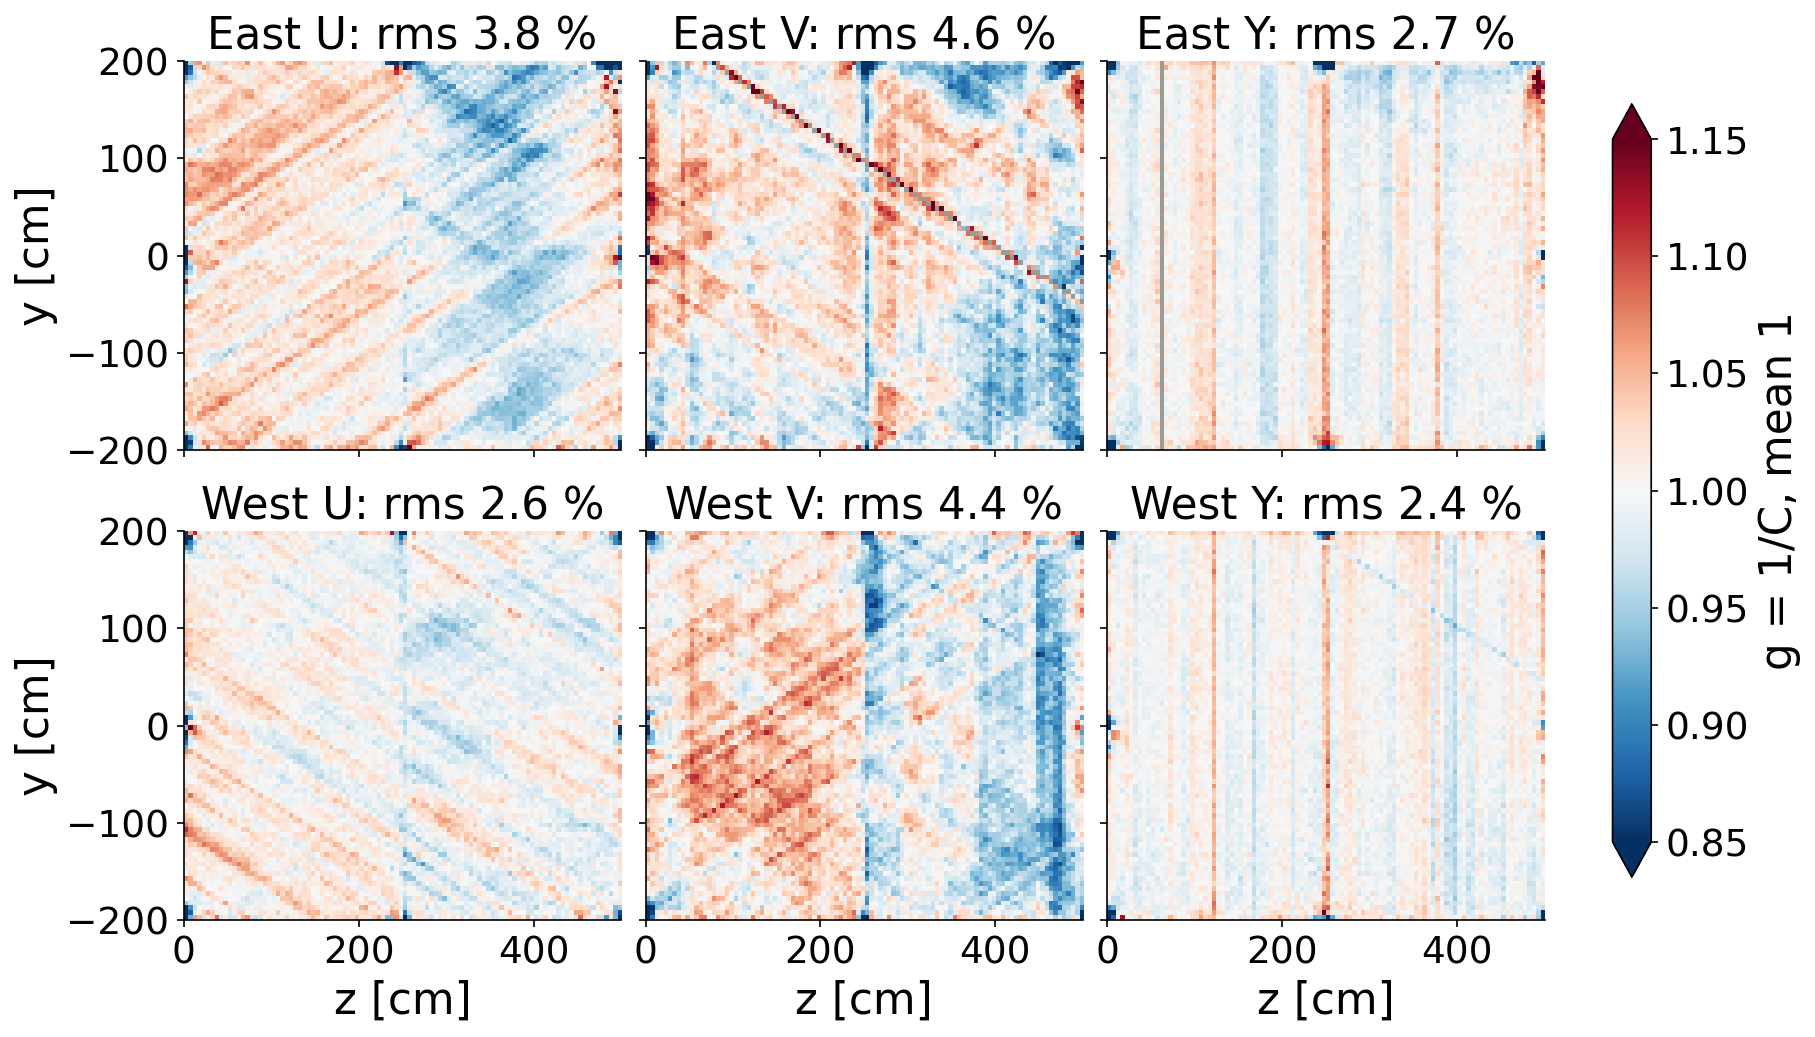
\includegraphics[width=0.78\textwidth]{fig_g_maps.png}\\[1mm]
\small
Red: more charge than the plane median. Gray: no data (factor 1 in the simulation).
rms over all pixels with data. Full range of the normalized factor: 0.42--1.68.
\end{frame}

% ---------------------------------------------------------------- 8
\begin{frame}{Non-uniformity in numbers (doc section 1)}
Good pixels: $C>0$ and $\ge$100 hits on all three planes. East 7,798 of 8,000; West 8,000.\\[2mm]
\centering
\begin{tabular}{@{}lrrrrrr@{}}
\toprule
 & East U & East V & East Y & West U & West V & West Y \\
\midrule
\multicolumn{7}{@{}l}{\footnotesize good pixels, $g = 1/C$:} \\
rms & 3.8\,\% & 4.3\,\% & 2.7\,\% & 2.6\,\% & 4.4\,\% & 2.4\,\% \\
5--95\,\% range & 0.94--1.05 & 0.93--1.06 & 0.97--1.04 & 0.97--1.03 & 0.92--1.06 & 0.97--1.03 \\
\midrule
\multicolumn{7}{@{}l}{\footnotesize all pixels with data, normalized $g$ (as in the simulation):} \\
rms & 3.8\,\% & 4.6\,\% & 2.7\,\% & 2.6\,\% & 4.4\,\% & 2.4\,\% \\
min -- max & 0.52--1.18 & 0.55--1.68 & 0.45--1.27 & 0.50--1.20 & 0.60--1.12 & 0.42--1.17 \\
\bottomrule
\end{tabular}
\raggedright
\vspace{3mm}
\begin{itemize}
\item V varies most on both TPCs; Y least.
\item East U varies more than West U (3.8 vs 2.6\,\%).
\item East V: 4.3\,\% on good pixels, 4.6\,\% on all. Dropping only its 64 pixels with $<$100 hits gives 4.3\,\%. The 1.68 maximum is one of them (3 hits, next to the empty diagonal).
\end{itemize}
\end{frame}

% ---------------------------------------------------------------- 9
\begin{frame}{Profiles along z and y}
\begin{columns}[c]
\begin{column}{0.62\textwidth}
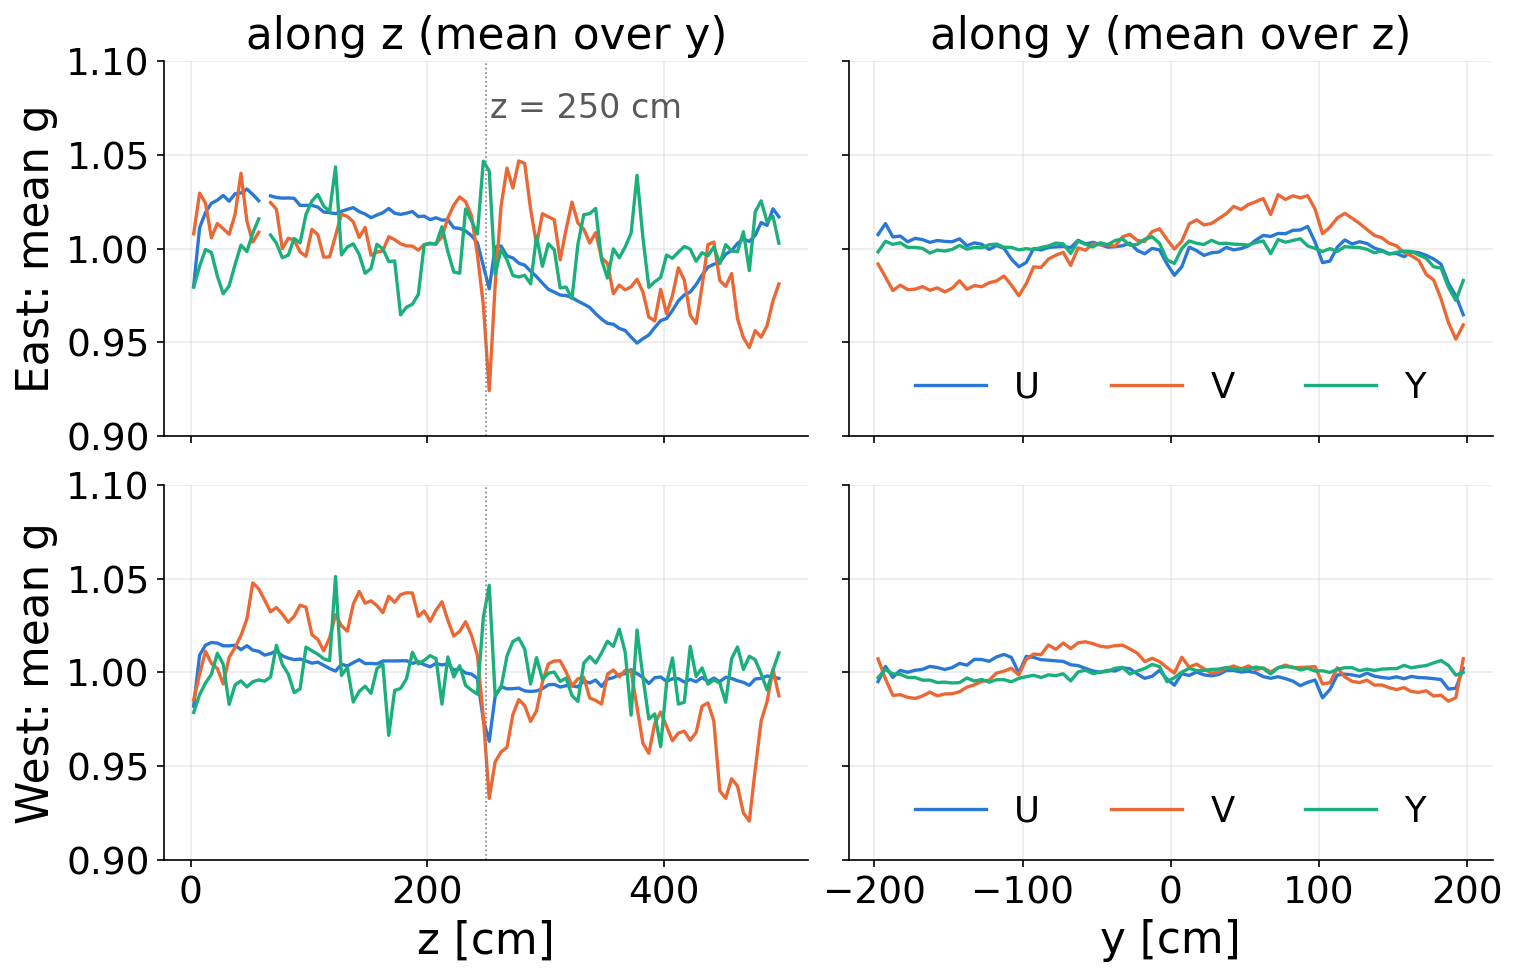
\includegraphics[width=\textwidth]{fig_profiles.png}\\
\footnotesize Mean of normalized $g$ over the good pixels.
\end{column}
\begin{column}{0.37\textwidth}
\footnotesize
\begin{itemize}
\item \textbf{z $\approx$ 250\,cm} (middle of the wire planes), both TPCs:
  \begin{itemize}
  \item U dips to 0.98 (East), 0.96 (West)
  \item V dips to 0.92, 0.93
  \item Y rises to 1.05, 1.05
  \end{itemize}
\item Large-scale trends along z: East U from 1.03 to 0.95 at z $\approx$ 380\,cm; V down to 0.92--0.95 at z $\approx$ 450--475\,cm.
\item Y along z: spikes on single 5\,cm columns.
\item Along y: within $\pm$2\,\% for U, Y and West V. East V goes from 0.98 (y $<$ $-$100\,cm) to 1.03 (y $\approx$ 80\,cm). East U and V fall to 0.96 at the top edge.
\end{itemize}
\end{column}
\end{columns}
\end{frame}

% ---------------------------------------------------------------- 10
\begin{frame}{Fine structure follows the wires}
\centering
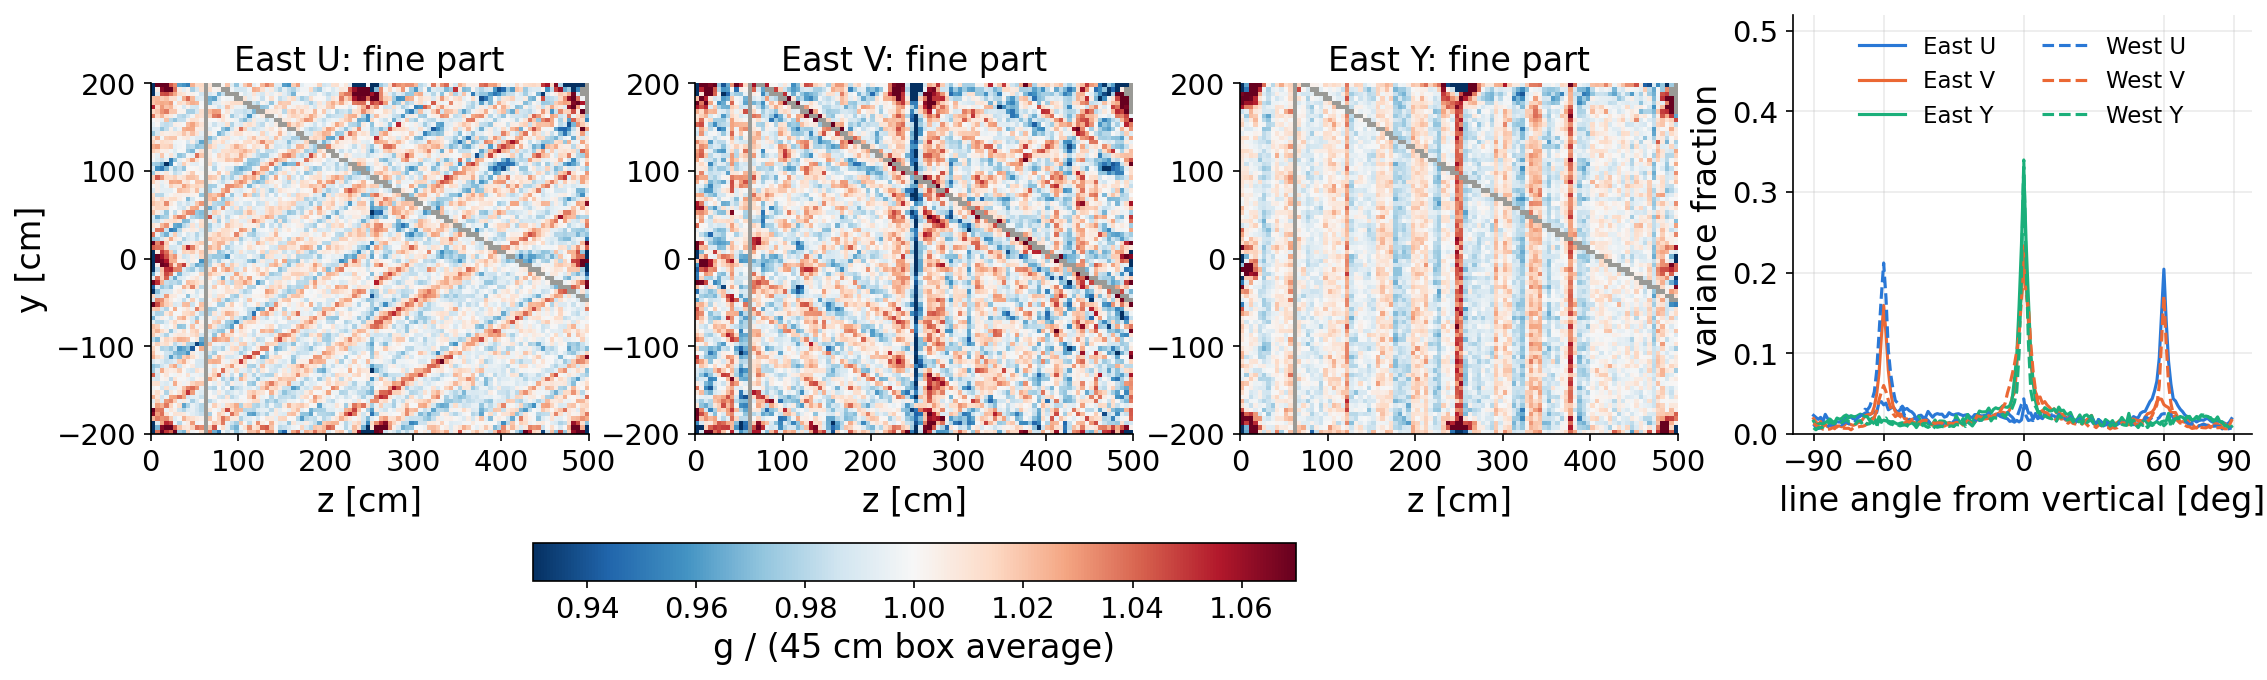
\includegraphics[width=\textwidth]{fig_stripes.png}\\[1mm]
\raggedright\footnotesize
Left: $g$ divided by its 45\,cm box average (East). Right: fraction of that fine part's variance that is constant along straight lines at a given angle from vertical.\\[1mm]
\begin{columns}[T]
\begin{column}{0.6\textwidth}
\begin{tabular}{@{}lrrrrrr@{}}
\toprule
fraction at & E U & E V & E Y & W U & W V & W Y \\
\midrule
$-60^\circ$ & 0.04 & \textbf{0.16} & 0.02 & \textbf{0.21} & 0.06 & 0.02 \\
$0^\circ$ (constant z) & 0.03 & \textbf{0.23} & \textbf{0.33} & 0.04 & \textbf{0.20} & \textbf{0.34} \\
$+60^\circ$ & \textbf{0.20} & 0.04 & 0.02 & 0.02 & \textbf{0.17} & 0.01 \\
\bottomrule
\end{tabular}
\end{column}
\begin{column}{0.38\textwidth}
\begin{itemize}
\item U: its wire direction only; the sign flips East/West.
\item Y: constant z.
\item V: its wire direction (East: along the empty diagonal) and constant z. The constant-z part is larger.
\end{itemize}
\end{column}
\end{columns}
\end{frame}

% ---------------------------------------------------------------- 11
\begin{frame}{Edges and corners}
\centering
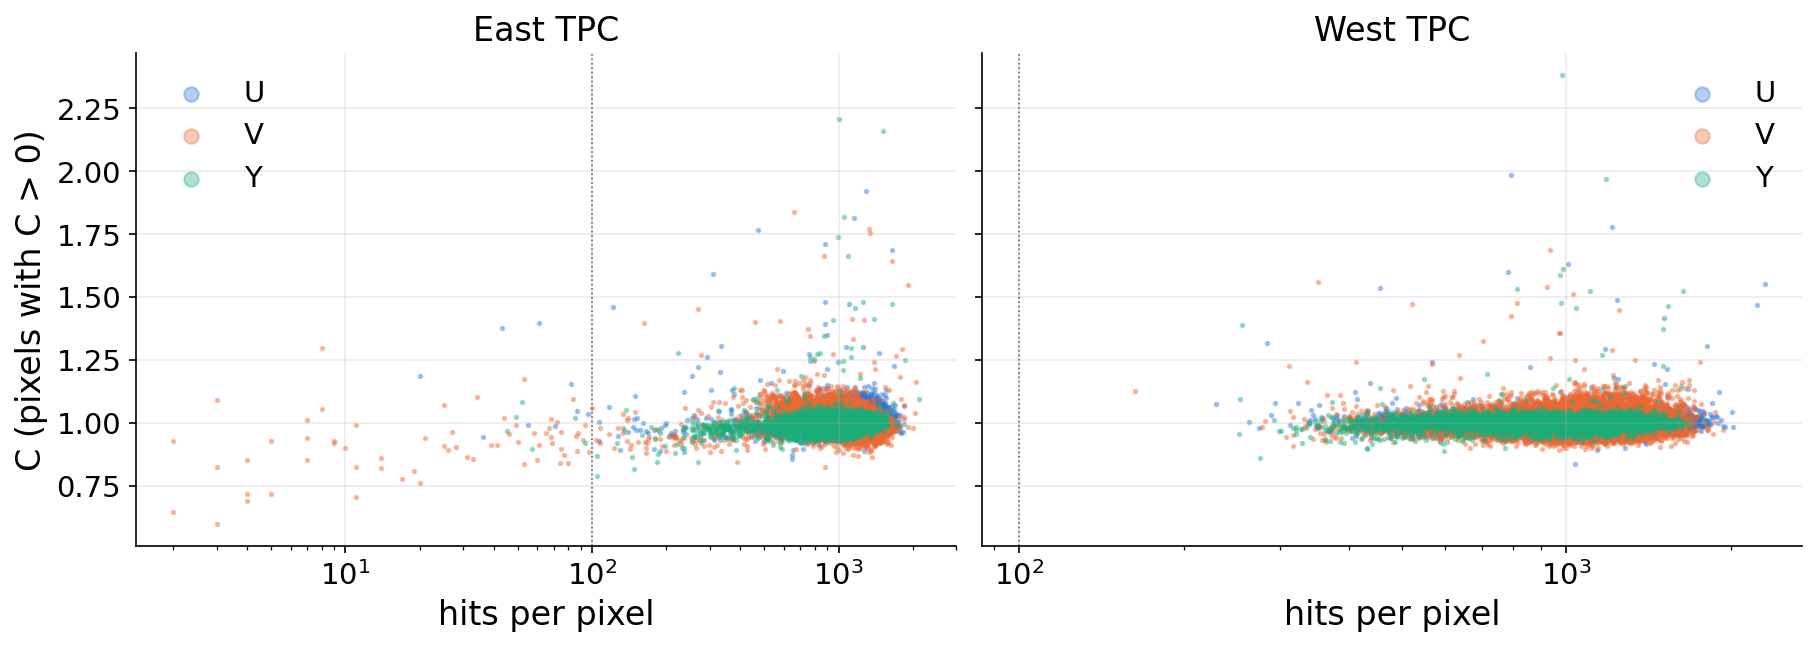
\includegraphics[width=0.8\textwidth]{fig_C_vs_hits.png}
\raggedright
\small
\begin{itemize}
\item Largest $C$ per plane and TPC: 1.69--2.38 (West Y 2.38, East Y 2.21). They sit at the corners (z 0--5\,cm, y $\pm$195--200\,cm) and at the top edge near z = 250\,cm.
\item All 11--15 pixels per plane with $C>1.3$ are in the outer 10\,cm. Their median is 870--1210 hits: \textbf{not} low statistics.
\item Pixels with $<$100 hits (East only) have $C$ = 0.60--1.40. 53 of the 64 East V ones touch the empty diagonal; the East U and Y ones are in the outer 10\,cm.
\item All are used as measured. If edges look wrong in the simulation, the converter can cap or fill them.
\end{itemize}
\end{frame}

% ---------------------------------------------------------------- 12
\begin{frame}{Plane to plane: one map for all planes does not work}
\begin{columns}[c]
\begin{column}{0.47\textwidth}
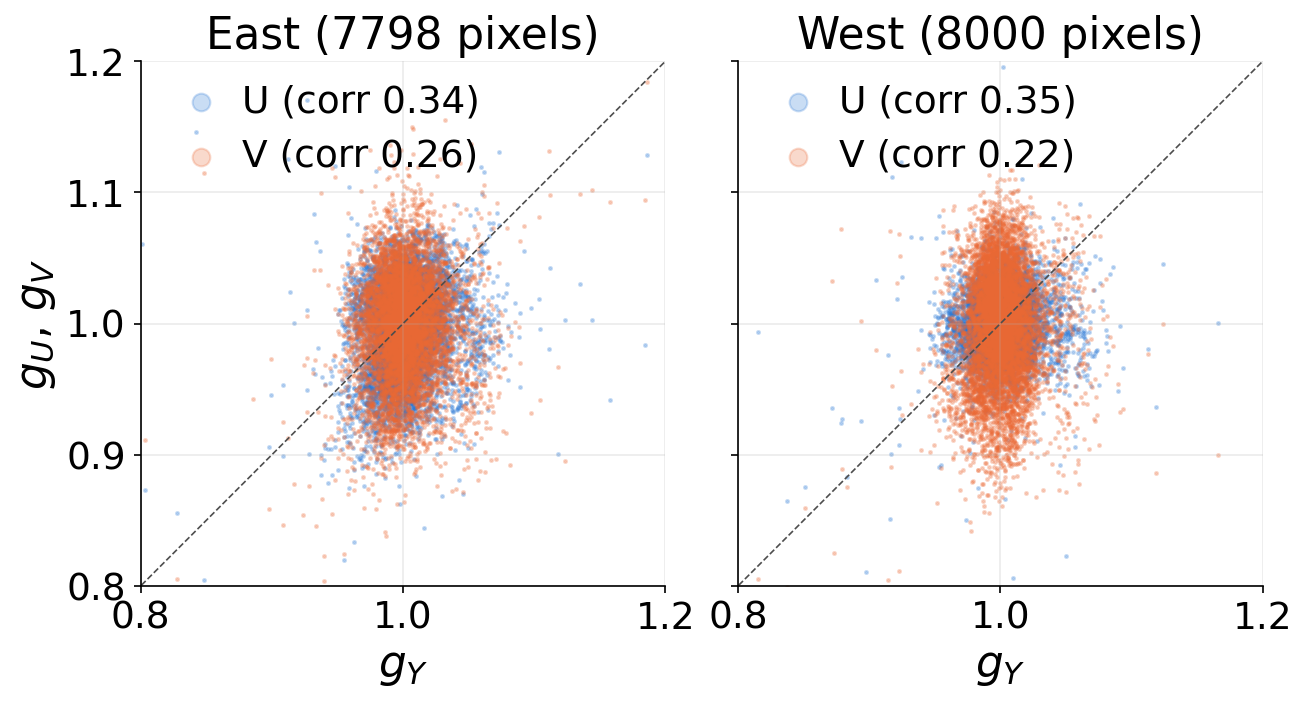
\includegraphics[width=\textwidth]{fig_plane_scatter.png}\\
\footnotesize Good pixels. Dashed line: equal response.
\end{column}
\begin{column}{0.52\textwidth}
\small
\begin{itemize}
\item Correlation between planes: 0.22--0.41 pixel by pixel; 0.25--0.51 on 45\,cm smoothed maps.
\item Plane-to-plane differences are as large as each plane's own variation.
\end{itemize}
\vspace{2mm}
\footnotesize\setlength{\tabcolsep}{3pt}
\begin{tabular}{@{}lrrrrrr@{}}
\toprule
rms of $g$ left [\%] & E U & E V & E Y & W U & W V & W Y \\
\midrule
no map & 3.8 & 4.3 & 2.7 & 2.6 & 4.4 & 2.4 \\
Y map for all planes & 3.9 & 4.5 & 0 & 2.9 & 4.5 & 0 \\
plane-average map & 2.4 & 2.8 & 2.3 & 1.8 & 2.7 & 2.2 \\
own map per plane & 0 & 0 & 0 & 0 & 0 & 0 \\
\bottomrule
\end{tabular}
\vspace{2mm}
\small
\begin{itemize}
\item The Y map does nothing for U and V.
\item The plane average removes about a third, and adds 2.2--2.3\,\% to Y.
\item $g_V/g_Y$ is off by $>$5\,\% in 24--26\,\% of the pixels.
\item \textbf{So: one factor per (plane, depo)}, as DepoTransformYZ does.
\end{itemize}
\end{column}
\end{columns}
\end{frame}

% ---------------------------------------------------------------- 13
\begin{frame}{Overall scale (data): the pixel medians}
\begin{columns}[c]
\begin{column}{0.56\textwidth}
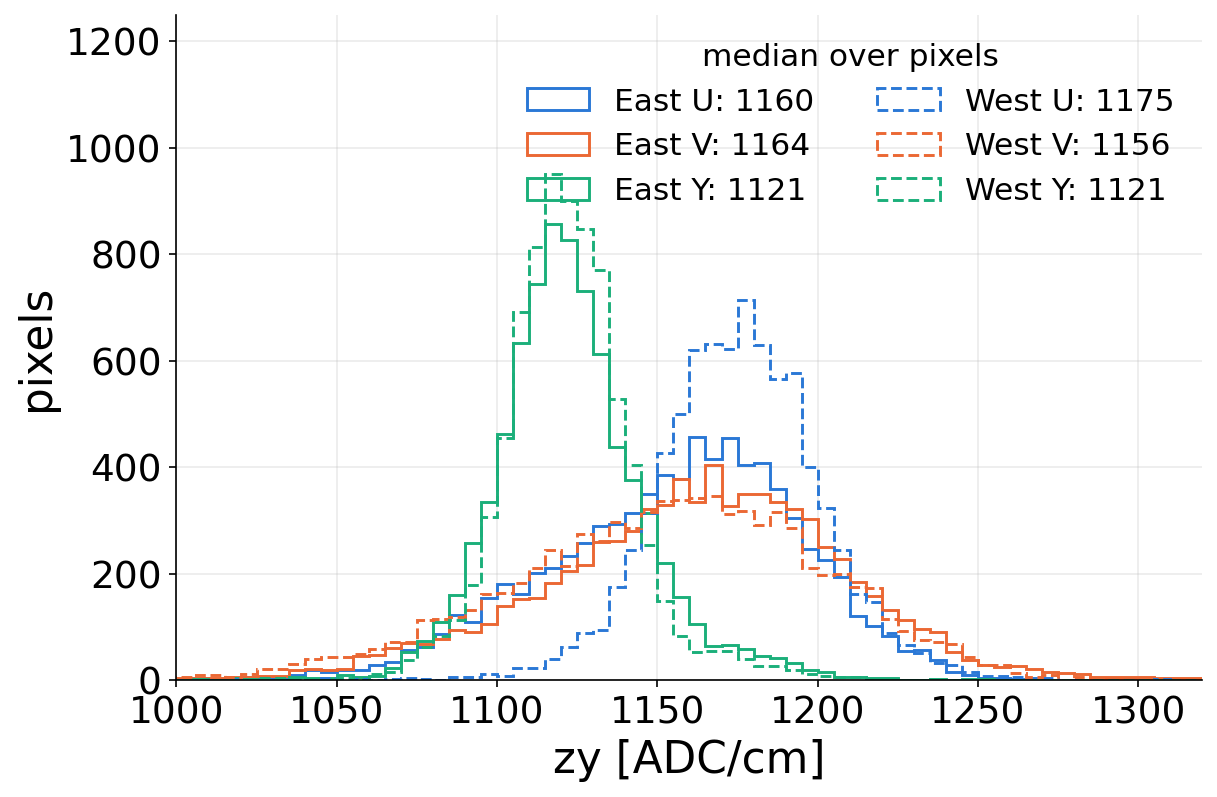
\includegraphics[width=\textwidth]{fig_zy_pixel_hist.png}
\end{column}
\begin{column}{0.43\textwidth}
\small
\code{zy} over the pixels of each plane and TPC; legend: median $M$ [ADC/cm].
\begin{itemize}
\item Y is below the induction planes:\\
  East: $-$3.3\,\% vs U, $-$3.7\,\% vs V\\
  West: $-$4.6\,\% vs U, $-$3.0\,\% vs V
\item West vs East:\\
  U +1.4\,\%, V $-$0.7\,\%, Y +0.02\,\%
\item The hit-weighted mean of \code{zy} gives West/East U +1.9\,\%, V $-$1.1\,\%, Y +0.04\,\%.
\item Y pixels spread less than U and V.
\end{itemize}
\end{column}
\end{columns}
\end{frame}

% ---------------------------------------------------------------- 14
\begin{frame}{Overall scale (data): 1D dQ/dx (\code{dqdxHist})}
\centering
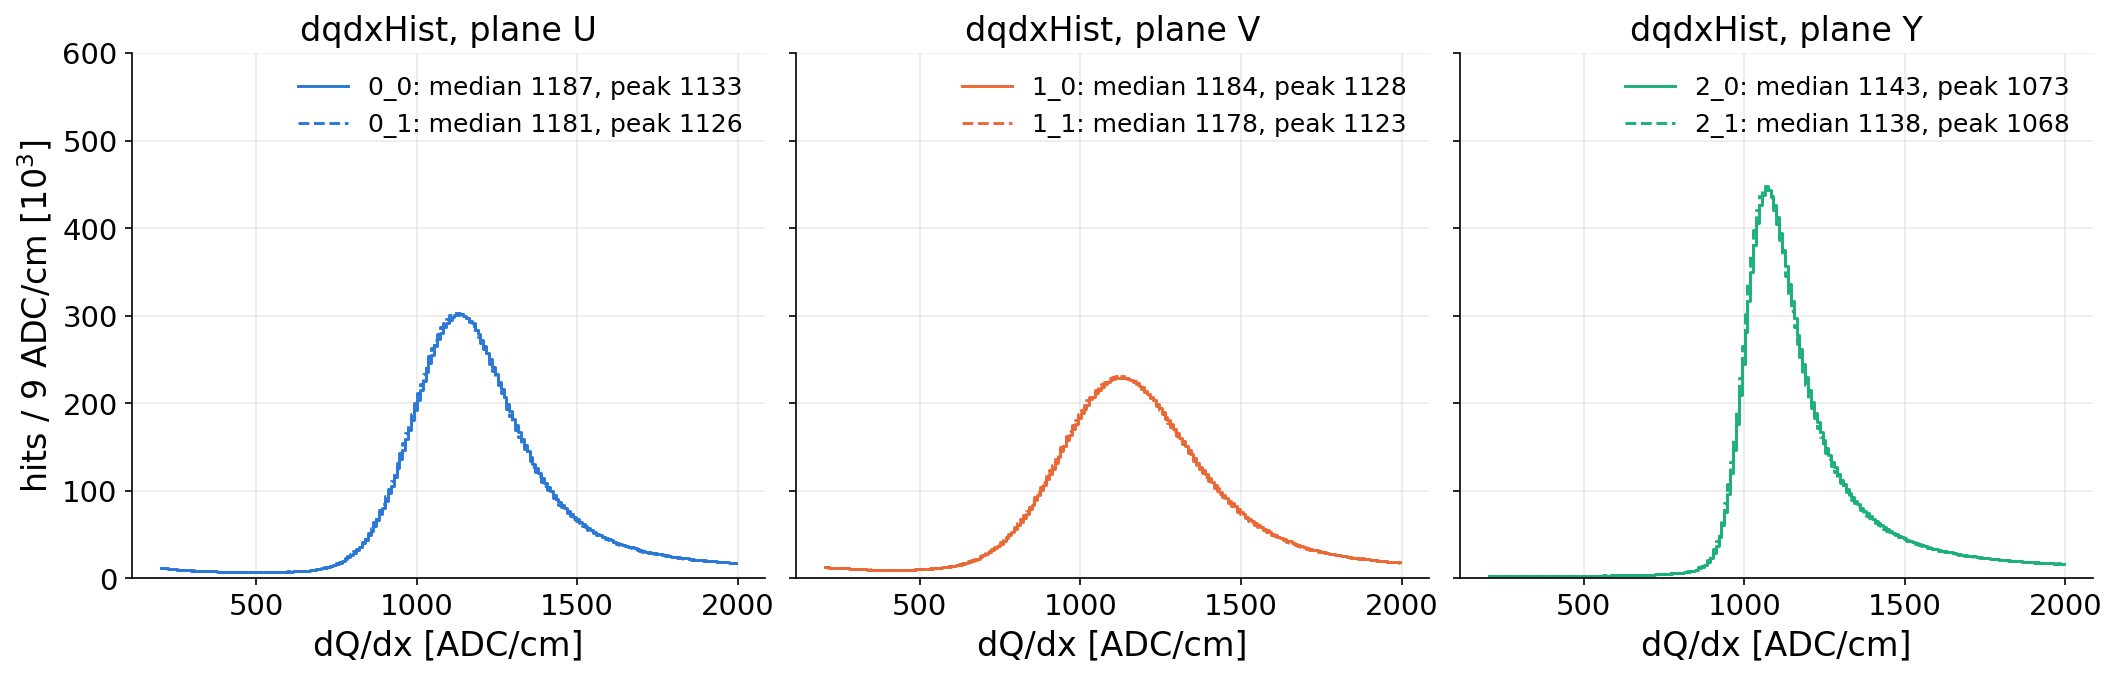
\includegraphics[width=0.96\textwidth]{fig_dqdx_1d.png}
\raggedright
\small
\begin{itemize}
\item Each \code{dqdxHist\_p\_t} has exactly as many entries as the East + West hits of that plane, e.g.\ U: 17,926,824 = 8,873,636 + 9,053,188. So \code{\_0} and \code{\_1} are \textbf{not} East and West.
\item \code{\_1} is 0.5\,\% lower than \code{\_0} (median, every plane). Their meaning is \open{a question for Kento}; we do not use them for East vs West.
\item Y vs U and V: peak 4.9--5.3\,\% lower, median 3.4--3.7\,\% lower.
\item 8--9\,\% of the entries are above 2000\,ADC/cm; 3\,\% (U, V) and 0.4\,\% (Y) below 200.
\end{itemize}
\end{frame}

% ---------------------------------------------------------------- 15
\begin{frame}{Overall scale (data): numbers}
dQ/dx in ADC/cm (unit from the 1D axis title; to confirm with Kento).\\[2mm]
\centering
\begin{tabular}{@{}lrr@{\hspace{8mm}}lrrrrr@{}}
\toprule
 & \multicolumn{2}{c}{\code{zy} over pixels} & & \multicolumn{5}{c}{\code{dqdxHist} (East + West hits)} \\
\cmidrule(r){2-3}\cmidrule(l){5-9}
 & median & hit-wt mean & hist & median & peak & mean* & $<$200 & $>$2000 \\
\midrule
East U & 1160 & 1153 & \code{0\_0} & 1187 & 1133 & 1195 & 3.2\,\% & 9.2\,\% \\
East V & 1164 & 1164 & \code{1\_0} & 1184 & 1128 & 1179 & 3.2\,\% & 9.2\,\% \\
East Y & 1121 & 1121 & \code{2\_0} & 1143 & 1073 & 1186 & 0.4\,\% & 8.3\,\% \\
West U & 1175 & 1174 & \code{0\_1} & 1181 & 1126 & 1189 & 3.2\,\% & 9.1\,\% \\
West V & 1156 & 1151 & \code{1\_1} & 1178 & 1123 & 1174 & 3.2\,\% & 9.0\,\% \\
West Y & 1121 & 1121 & \code{2\_1} & 1138 & 1068 & 1181 & 0.4\,\% & 8.2\,\% \\
\bottomrule
\end{tabular}\\[1mm]
\raggedright\footnotesize
\code{dqdxHist} median includes under- and overflow. Peak: parabola over the 7 bins around the maximum (bins of 9\,ADC/cm). *Mean over 200--2000 only, so biased by the range.\\[3mm]
\small
\begin{itemize}
\item In data, Y is 3--5\,\% below U and V. East and West differ by 0.7--1.9\,\% for U and V, $<$0.05\,\% for Y.
\item The normalized map carries none of this: it gives shape only.
\item \open{Data vs MC overall scale: open.} It needs the same histograms from MC (same selection and binning). We have no MC numbers.
\end{itemize}
\end{frame}

% ---------------------------------------------------------------- 16
\begin{frame}{Validation (doc section 3)}
\small
\begin{itemize}
\item Doctest: lookups, edge clamp, grid checks, per-plane scaling of one depo (ratios equal within $10^{-4}$), unit map = \code{DepoTransform}. 5/5 cases, 412 assertions. Before the YZMap fix: a wrong value, then SIGSEGV.
\item 10 long 5\,GeV $\mu^-$ (along +z, $\pm$20$^\circ$ in YZ); detsim nominal vs yzmap, same build, 5:11 wall each. Per channel: SP charge ratio vs the map factor predicted from its SimChannel IDEs; 18,489 channel-events with $\ge$20,000 electrons.
\end{itemize}
\vspace{1mm}
\centering
\footnotesize
\begin{tabular}{@{}lrrrrrr@{}}
\toprule
 & channels & predicted rms & meas/pred $-$1: median & rms & corr & total meas / pred \\
\midrule
East U & 4150 & 3.5\,\% & $-$0.01\,\% & 2.2\,\% & 0.83 & 0.9995 / 0.9997 \\
East V & 6298 & 3.8\,\% & $-$0.13\,\% & 3.0\,\% & 0.74 & 1.0034 / 1.0050 \\
East Y & 2404 & 1.9\,\% & +0.00\,\% & 0.75\,\% & 0.93 & 0.9972 / 0.9973 \\
West U & 2228 & 2.3\,\% & $-$0.01\,\% & 2.6\,\% & 0.65 & 0.9988 / 0.9991 \\
West V & 2274 & 4.4\,\% & $-$0.10\,\% & 3.5\,\% & 0.73 & 1.0002 / 1.0028 \\
West Y & 1135 & 1.8\,\% & +0.01\,\% & 0.49\,\% & 0.96 & 0.9983 / 0.9985 \\
\bottomrule
\end{tabular}
\raggedright
\small
\begin{itemize}
\item Each plane follows its own map: median deviation $\le$0.13\,\%, plane totals within 0.3\,\%.
\item Collection within 0.5--0.75\,\% rms; induction 2--3.5\,\% (noise, small per-channel charge).
\end{itemize}
\end{frame}

% ---------------------------------------------------------------- 17
\begin{frame}{Open questions for Kento, next steps}
\small
\textbf{Questions for Kento}
\begin{enumerate}
\item \textbf{Unit and stage} of \code{zy}: ADC/cm as on the 1D axis? After which corrections?
\item \textbf{``200usEast80usWest''}: what is it? A time or drift cut per TPC? Why different for East and West?
\item \textbf{\code{dqdxHist\_p\_0} vs \code{\_p\_1}}: both hold East + West hits, \code{\_1} is 0.5\,\% lower. What is each?
\item \textbf{MC version} of the same histograms, for the data/MC overall scale per plane and TPC.
\item \textbf{Outer 10\,cm}: are $C$ = 1.7--2.4 there real, or a selection effect? Cap them?
\item \textbf{Selection}: which tracks and hits, run range, number of events? Later versions planned?
\item \code{zydqdx}: intended content? (NaN in 806--5160 pixels.)
\end{enumerate}
\vspace{2mm}
\textbf{Next steps on our side}
\begin{itemize}
\item Map file committed to wire-cell-data master (acbe8e5, 2026-11-24).
\item Possibly a YZ-map variant of the sbndcode jsonnet (with DNN ROI); the current one starts from the older toolkit copy.
\item Data/MC overall scale once the MC histograms exist.
\end{itemize}
\end{frame}

% ---------------------------------------------------------------- 18
\begin{frame}{Summary}
\begin{itemize}
\item Kento's file gives, per plane and TPC, the median dQ/dx in 5\,cm $\times$ 5\,cm YZ pixels and $C$ = (plane median) / (pixel median). Data only.
\item Coverage: median 980--1170 hits per pixel. Empty pixels only on East (V diagonal 52, Y column 80).
\item Non-uniformity rms: U 2.6--3.8\,\%, V 4.3--4.6\,\%, Y 2.4--2.7\,\%. The structure follows each plane's wires, plus the z $\approx$ 250\,cm line and the outer 10\,cm.
\item Planes are weakly correlated (0.2--0.4). One factor per depo cannot serve all planes. The simulation scales each depo per plane (DepoTransformYZ); validated with single muons.
\item Data scale: Y is 3--5\,\% below U and V; East and West agree within 2\,\%. The data/MC overall scale is open and needs Kento's MC histograms.
\end{itemize}
\end{frame}

\end{document}
